\begin{multicols}{2}
\cappar Eu João Afonso Gaspar do Amaral, filho de José e Maria Gaspar Fernandes Afonso Domingos, nascido em Luanda em 19 abril de 1994 residentes em Vila Alice. Vivo em uma casa  humilde na vila alice com o meu avô e meus tios, que sempre foram uma das forças para o xadrez seja uma realidade  em minha vida. 

\begin{figurebox}
 \vspace{20pt}
 \centering
 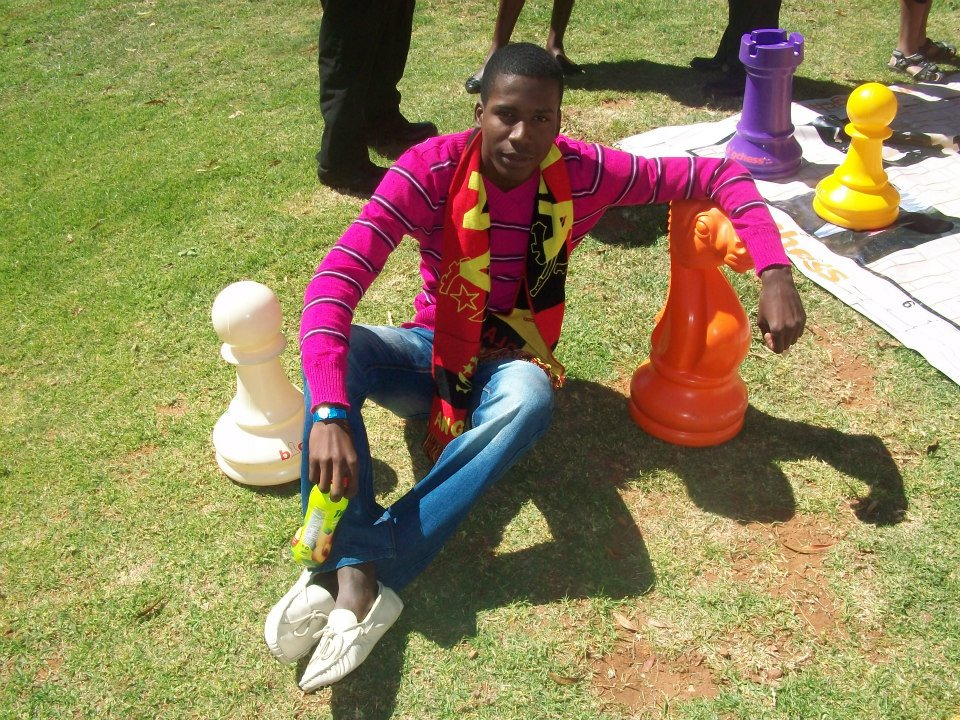
\includegraphics[scale=0.22]{jugando2.jpg}\\
 João Afonso Gaspar Do Amaral\\ 
 {\small Xadrez Jovem Angolano}
 \vspace{1pt}
  %\vspace{0.1\textheight}
\end{figurebox}
\textbf{Formação académica}

Frequento o Instituto normal de Educação Marista a 13ª classe no curso de Física Matemática, eu tive minha formação básica na escola Magistério primário, já no ensino médio a vida e o xadrez me fez escolher o curso Mat-Física, devido à facilidade com as ciências do raciocínio lógico,neste momento sou um dos finalistas desta escola  de educação e é muito importante notar que durante a minha vida académica o xadrez sempre foi a base para o desenvolvimento do nível académico em todos sectores.

\textbf{Minha Trajectória xadrezistica}

 Minha carreira xadrezistica tem sido a base da formação da minha personalidade, começar dizendo que meu primeiro contacto com o xadrez foi quando eu tinha 10 anos , a convite de um amigo Vanderson dias um grande amigo de infância fomos atraídos pela belas peças de xadrez e os belos movimentos das peças, isso aconteceu em um Largo da Vila Alice, com a vontade de aprender a jogar xadrez fomos convidados a conhecer o desporto ciência pelo  Sr. Abilio Silva ( locas ) , aparte desta data criou-se um núcleo de xadrez que passou a se chamar Núcleo da Vila Alice criado no ano de 2004, com o meu desejo de aprender a se tornar um jogador de xadrez profissional fui aprendendo as primeiras bases do xadrez , no ano 2005 fiz minha primeira participação em um campeonato profissional na categoria de juvenil que se realizou em Benguela como primeiro ano foi a experiência que valeu neste ano, em 2006 foi bom porque tive uma maior participação em diversos torneios nacionais e campeonatos também foi este ano que este núcleo Vila Alice começou a ter  jogadores de boa qualidade e também a se destacar entre as grandes equipas de Angola, embora não tem um elevado número de os jogadores mais  tinha uma boa qualidade na formação dos jogadores e é chamado por muitos como um Núcleo de Campeões , em 2007 procurei levar o xadrez como base central na minha vida ou melhor algo que poderia lançar-me para a vida como um bom homem e sempre com apoio da minha família , amigos e Senhores que gostavam do desporto ciência tal como o Sr Abilio Silva e também nesta ano  sai em 3 º lugar no Campeonato Nacional da Juvenil e boas classificações em outros torneios , em 2008, continuou a crescer vontade de aprender  xadrez e desenvolver a minha juventude com o xadrez, no ano de 2009  foi bom com muitas vitorias e glórias  neste ano fui campeão no Campeonato Nacional e Provincial de Juvenil  2009 com muita classe,determinação ,disciplina, com a ajuda dos meus treinadores (locas e Garrido) e as pessoas que tornaram possível a minha presença nestes campeonatos ,o Campeonato Nacional foi realizado na província de Malanje com essa vitoria desencadeou a minha primeira chamada na selecção Nacional de xadrez de Júnior para participar no Campeonato Mundial na Argentina ( Portun Madryn ) aparte deste Mundial comecei com minha carreira internacional que foi muito importante na minha vida xadrezistiica desde então, até hoje, foi uma luta de poder desenvolver no mundo do xadrez internacional e Nacional, em 2011 foi participar no Campeonato Africano da Juventude na África do Sul onde obtive o 4ºLugar depois de muita luta com jogadores de nível muito difícil visto que a formação xadrezistica e didáctica é melhor que em Angola, em 2012 eu participei do Open Sul-Africano , em Pretória , onde em 9 jogos vencei 7 jogos e perdeu apenas 2 jogos, no em 2013 eu participei no torneio internacional Benirdom na Espanha, esse Torneio foi a melhor experiência da minha vida e poder realizar o sonho de poder jogar na grande montra do xadrez mundial que é a Espanha.....nesta minha trajectória sempre foi possível com ajudar de amigos, familiares e outras pessoas que acompanharam o meu desenvolvimento no xadrez, para dizer como eu sempre tive o Núcleo Vila Alice mais este ano de 2014 tive a honra de Jogar pela Escola IMNE - Marista ( Cristo Rei ) uma oportunidade que me foi dada pelo Ir. Jesus .

\begin{center}
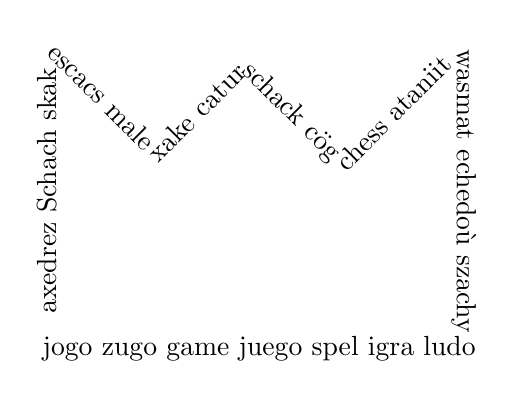
\begin{tikzpicture}
\path node at (0,0) [rotate=90] {axedrez Schach skak} 
      node at (0.7,1.2) [rotate=-45]{escacs male}
      node at (1.9,1) [rotate=45]{xake catur}
      node at (3.1,1) [rotate=-45]{schack c\"og}
      node at (4.4,1) [rotate=45]{chess ataniit}
      node at (5.3,0) [rotate=-90] {wasmat echedoù szachy}
      node at (2.7,-2) {jogo zugo game juego spel igra ludo} 
;
\end{tikzpicture}
\end{center}

\textbf{Meus Sonhos e os benefícios do xadrez na minha vida}

Meu sonho no xadrez e com o xadrez sempre foi tornar com o xadrez  Angola um pais melhor para se viver e poder construir bons homens para sociedade Angolana, como todo  jovem há um sonho particular que nasce dentro de cada um e meu sonho é baseado em minha formação e jogador Académica e a minha formação no xadrez de forma a tornar-me um Mestre Internacional até mesmo um Grande Mestre mais isso só é possível com um investimento e uma formação, sempre sonhei e espero ter uma bolsa de estudos para completar a minha formação académica e xadrezistica é importante  dizer  que não é um bom jogador de xadrez sem uma formação de qualidade tanto formação Académica e xadrezistica por isso sempre sonhei em uma bolsa de estudo neste momento é o meu principal foco com objectivo de desenvolver o meu xadrez e se formar para ajudar no desenvolver o país,nesta oportunidade vejo a forma solicitar uma bolsa de estudo , Actualmente estou terminando médio na Escola de Formação de Professores IMNE-MARISTA no curso de Mat-Fisica e sinto que estou preparado para o desafio de uma bolsa de estudo e o aperfeiçoamento do meu xadrez , sempre sonhei na Espanha como um país para minha formação no xadrez e académica devido a qualidade de ensino do xadrez e boas universidades a nível académico, pela impossibilidade financeira solicito aquém poder  ajudar a minha Formação xadrezistica e a minha formação académica , eu também quero falar dos benefícios que o xadrez Troce na minha vida em todos os aspectos começando pela Área  Académica dizer que o xadrez tornou-me uma pessoa mais organizada com materiais escolares, bom raciocínio lógico nas ciências exactas como: matemática , Física e química, não só outros também, na área social o xadrez me ajudou a viver em sociedade, a cumprir as normas sociais e melhorar a minha relação com os outros, no campo económico o xadrez me ajuda a ganhar mais controle e gerência dos minhas coisas, obter ideias e formas de investimento para uma melhor desenvolver alguns bens e me ensinou a ser disciplinado com a ajuda de duas grandes pessoas o Sr. Abilio Silva e irmão de Jesus.

\textbf{Conselho para Crianças e do Pais de xadrez}
 
O meu conselho vai para os pais de cada criança para motivar e levar as crianças para a prática de xadrez será um grande benefício para o desenvolvimento saudável de seus filhos, o xadrez vai ajudar em vários aspectos da criança como me ajudou em geral alguns dos benefícios para as crianças são: uma melhor dinâmica na criança, melhor interacção da criança com a sociedade, desenvolvimento da Capacidade de raciocínio da criança, em alguns casos ajudar as crianças a superar  traumas que vive em casa ou obteve na sociedade, e desenvolver o poder de interpretar na escola e alguns fenómenos, desenvolvimento rápido de  alguns órgãos como a fala, a visão e outros. Os Benefícios que xadrez traz nas crianças são milhares , por isso deixo o conselho para cada Encarregado de educação para deixar seu filho no belo mundo de xadrez.

Quero agradecer a Deus em primeiro lugar e a oportunidade que a Revista Soluções me beneficiou , o Sr. Abilio Silva, o Sr. Antonio Yuz, Ir.Jesus, o Sr. David Adão, minha família e amigos, a Sra. Maria, o meu apreço pela oportunidades que me deram para poder desenvolver o xadrez na minha  vida.

Graciosamente 

    João Amaral

\end{multicols}
\begin{center}
  \begin{figurebox}
 \begin{center}  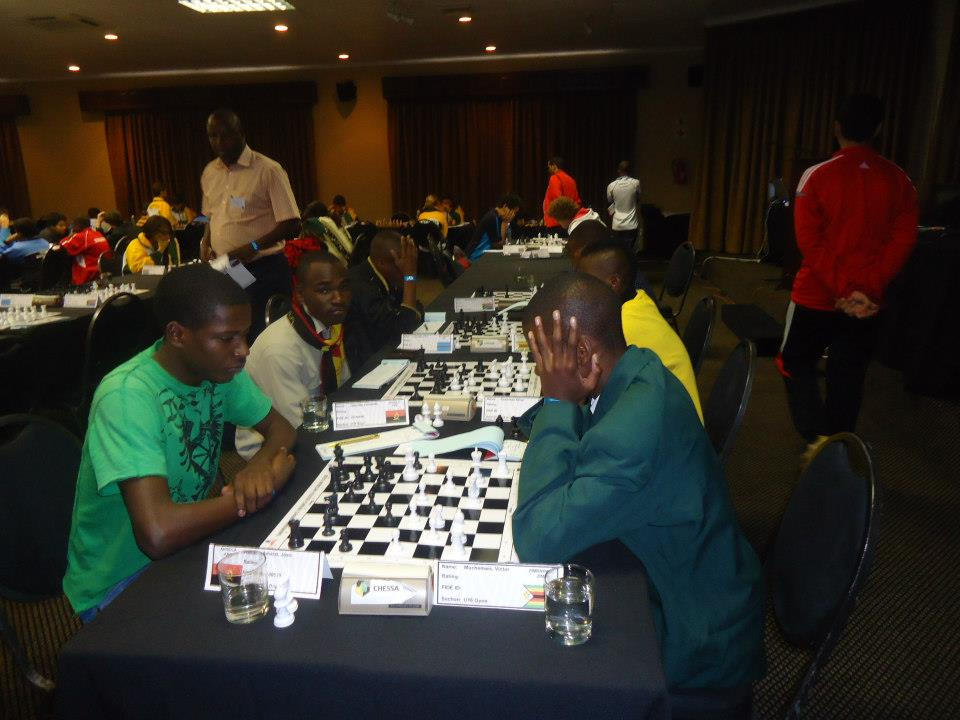
\includegraphics[scale=0.2]{jugando3.jpg}
   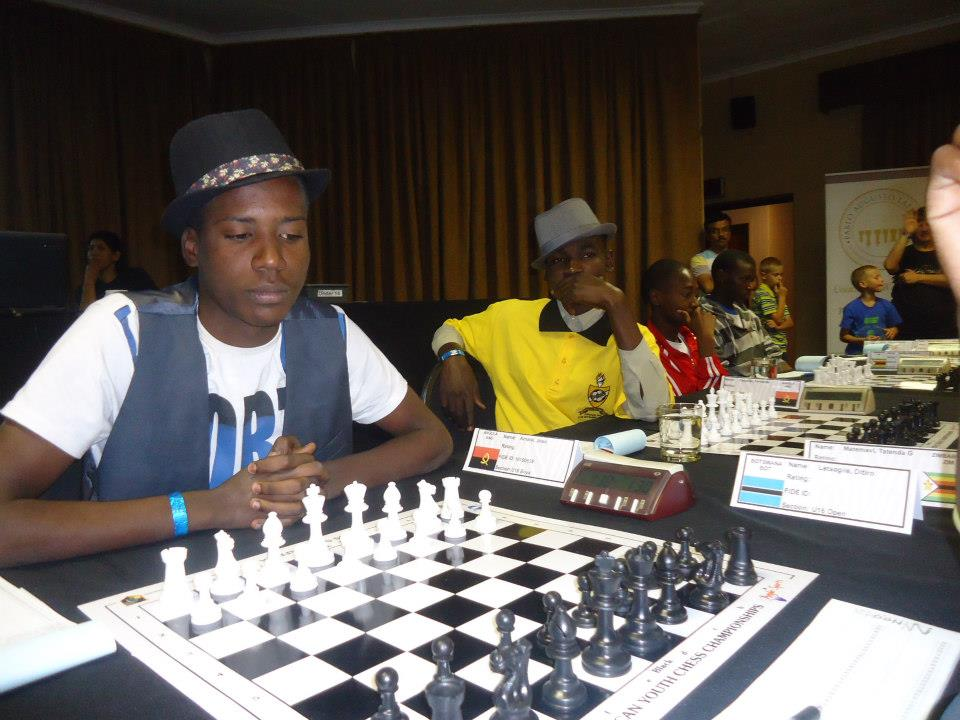
\includegraphics[scale=0.2]{fotoJoao.jpg}\end{center}
 \begin{center}  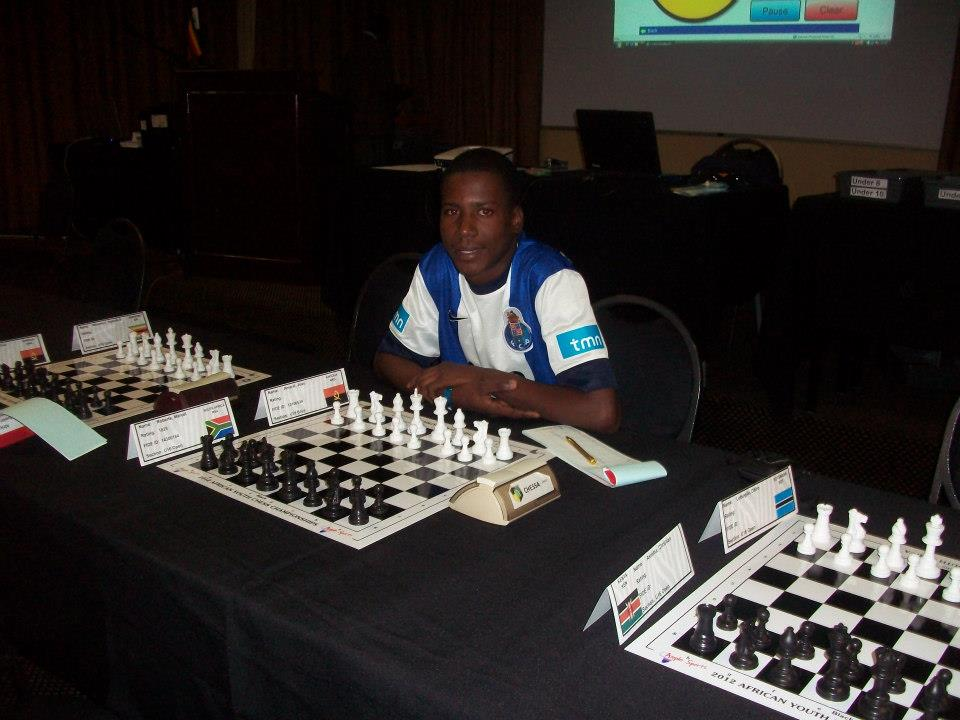
\includegraphics[scale=0.2]{fotoJoao2.jpg}
  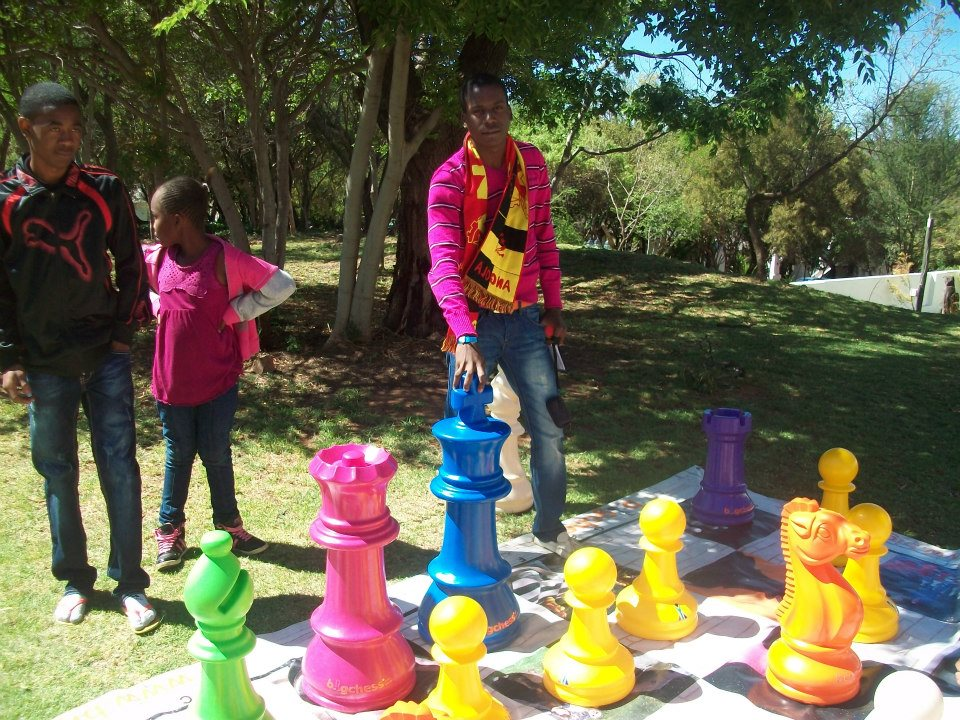
\includegraphics[scale=0.2]{jugando1.jpg}\end{center}
\centering João Amaral jugando.
 \end{figurebox}
\end{center}

%\vspace{3cm}
\noindent
\centering
\includegraphics[scale=0.5]{pubmm.png}


\newpage

%%% Local Variables: 
%%% mode: latex
%%% TeX-master: "solucionenaccion"
%%% End: 



